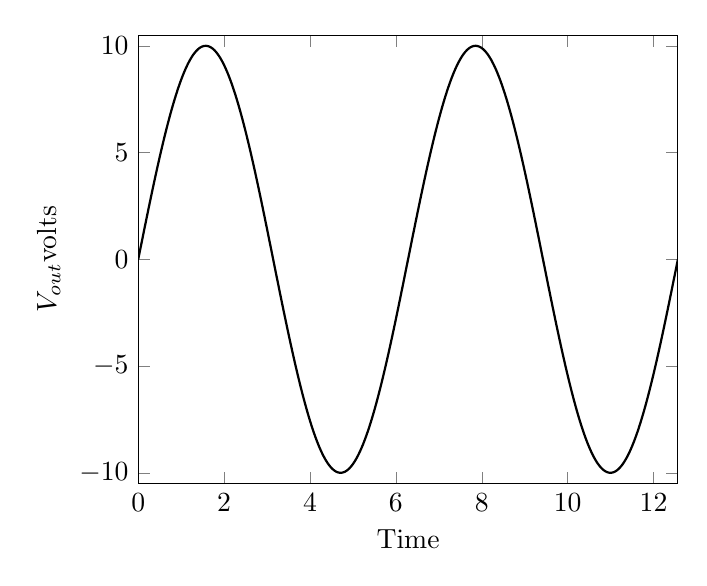
\begin{tikzpicture}
\begin{axis}[
    xlabel=Time,
    ylabel={$V_{out}$\brak{volts}},
    xmax=4*pi, xmin=0, 
    ymax=10.5, ymin=-10.5, % Adjust these values according to your data range
    ytick={-10,-5,0,5,10}, % Adjust these values according to your data range
    yticklabels={$-10$,$-5$,$0$,$5$,$10$}, % Adjust these values according to your data range
]
\addplot[domain=0:4*pi, samples=400, black, thick]{10*sin(deg(x))};
\end{axis}
\end{tikzpicture}
